\documentclass[10pt]{article}
\usepackage[utf8]{inputenc}
\usepackage[english]{babel}
\usepackage[font=small,labelfont=bf]{caption}
\usepackage{geometry}
\usepackage{natbib}
\usepackage{pxfonts}
\usepackage{graphicx}
\usepackage{newfloat}
\usepackage{setspace}
\usepackage{hyperref}
\usepackage{placeins}
\usepackage{booktabs}
\usepackage{longtable}

\newcommand{\argmax}{\mathop{\mathrm{argmax}}\limits}
\newcommand{\argmin}{\mathop{\mathrm{argmin}}\limits}

\newcommand{\knowledgeMaps}{5}

\title{\textit{Supplementary materials for}: Text embedding models yield high
resolution insights into conceptual knowledge from short multiple choice
quizzes}

\author{Paxton C. Fitzpatrick\textsuperscript{1},
Andrew C. Heusser\textsuperscript{1, 2}, and Jeremy R.
Manning\textsuperscript{1, *}\\\small{\textsuperscript{1}Department of Psychological and Brain Sciences}\\\small{Dartmouth College, Hanover, NH 03755, USA}\\\small{\textsuperscript{2}Akili Interactive Labs}\\\small{Boston, MA 02110, USA}\\\small{\textsuperscript{*}Corresponding author:
Jeremy.R.Manning@Dartmouth.edu}}

\date{}

\begin{document}

\renewcommand{\figurename}{Supplementary Figure}

\setcounter{equation}{0}
\setcounter{figure}{0}
\setcounter{table}{0}
\setcounter{page}{1}
\setcounter{section}{0}
\makeatletter
\renewcommand{\theequation}{S\arabic{equation}}
\renewcommand{\thefigure}{S\arabic{figure}}
\renewcommand{\thetable}{S\arabic{table}}
\renewcommand{\bibnumfmt}[1]{[S#1]}
\renewcommand{\citenumfont}[1]{S#1}

\newcommand{\topics}{3}

% \newcommand{\demo}{1}

\begin{titlepage}
\maketitle
\end{titlepage}

\begin{tiny}
\renewcommand*{\arraystretch}{1.4}
\begin{longtable}{r|p{0.375in}|p{1.275in}|p{0.75in}|p{0.75in}|p{0.75in}|p{0.75in}}

    
    \textbf{ID} & \textbf{Question set} &                                                                                                                                                                                                                                                                         \textbf{Question} &                                                                                                                                     \textbf{Correct response} &                                                                                                     \textbf{Alternative 1} &                                                                                                                          \textbf{Alternative 2} &                                                                                                                                 \textbf{Alternative 3} \\\hline
    1     &     FFF &                                                                                                                                                                                   Why is the gravitational attraction between you and your computer too small for you to notice? &                                           Neither you nor your computer has enough mass to cause a noticable gravitational attraction &                You and your computer are too close for the gravitational attraction to be significant &                                                                        Humans are too small to detect the force of gravity &  The gravitational attraction between you and your computer is disrupted by the larger gravitational field generated by the earth \\\hline
    2     &     FFF &                                                                                                                                                                                                                    Which of the following is an example of the Weak Interaction? &                          A neutron in a radioactive Cesium atom is converted into a proton, leading to the release of a few particles &  Light from the sun collides with a satellite orbiting Earth and exerts a small push on the satellite &  Two protons bound together in a Helium nucleus resist separation despite a repulsive electromagnetic force acting on them &                                                   A distant galaxy exerts a small but detectable gravitational pull on the  Earth \\\hline
    3     &     FFF &                                                                                                                                                                                                            Roughly how many times stronger is the Weak Interaction than gravity? &                                                                                                    10,\-000,\-000,\-000,\-000,\-000,\-000,\-000,\-000 &                                                                                                    10 &                                                                                                                  1,000,000 &                                                                                  The Weak Interaction is less strong than gravity \\\hline
    4     &     FFF &                                                                                                                                                                              Why don't you and your computer experience any attraction or repulsion due to the Weak Interaction? &                                                                         The weak interaction only acts over extremely small distances &                The weak interaction between you and your computer is counteracted by the other forces &                                                                                   You and your computer have no net charge &                                            Neither you nor your computer has enough mass to induce a significant Weak Interaction \\\hline
    5     &     FFF &                                                                                                                                                                                            Which of the following is a difference between gravity and the electromagnetic force? &                                            Gravity is only ever attractive while the electromagnetic force can both attract and repel &                                           Gravity is a much more powerful force than electromagnetism &           Gravity can only act over large distances while the electromagnetic force can act over large and small distances &                   The electromagnetic force can only act over small distances while gravity can act over small or large distances \\\hline
    6     &     FFF &                                                                                                                                                                                                  Electricity and magnetism can be shown to be two cases of the same force if we: &                                                                                            View them in different frames of reference &                              Switch which charges we call positive and which charges we call negative &                                        Consider both the effects over small distances and the effects over large distances &                                                           Consider both the attractive and repulsive properties of the two forces \\\hline
    7     &     FFF &                                                                                                                                  Which of the following are the primary two fundamental forces acting in opposition between the positively-charged protons in an atom's nucleus? &                                                                                        The Strong Force and the Electromagnetic Force &                                                                      Gravity and the Weak Interaction &                                                                                      Gravity and the Electromagnetic Force &                                                                                         The Strong Force and the Weak Interaction \\\hline
    8     &     FFF &                                                                                                                                                                     Why does the universe have a very uneven distribution of mass but a relatively equal distribution of charge? &  Positive and negative charges cancel out and become a neutral charge when they combine while masses only grow larger as they combine &                                                    Masses tend to repel while charges tend to attract &                                                                         Masses tend to attract while charges tend to repel &       The gravitational interaction acting between masses is stronger than the electromagnetic interaction acting between charges \\\hline
    9     &     FFF &  In your body, there are a tremendous amount of negatively-charged electrons. Your computer also contains a huge number of negatively-charged electrons. We know that like charges repel, but you and your computer are not repelled apart. Which of the following explains why? &                                    The electrons' negative charges are balanced by the positive charges of an equal number of protons &                                         An attractive gravitational force balances out this repulsion &                                                              The Electromagnetic force only acts over very small distances &                                                                     The Electromagnetic force only acts over very large distances \\\hline
    10    &     FFF &                                                                                                                                                                                        Which of the following is a similarity between the Weak Interaction and the Strong Force? &                                                                                               Both act only over very small distances &                                                      Both are stronger than the Electromagnetic force &                                                                                               Both are weaker than Gravity &                                                                     Both are responsible for attractions between distant galaxies \\\hline
    11    &     FFF &                                                                                                                                                                                                                          Which force is stronger than the Electromagnetic Force? &                                                                                                                          Strong Force &                                                                                               Gravity &                                                                                                           Weak Interaction &                                                                                            Electromagnetic Force is the strongest \\\hline
    12    &     FFF &                                                                                                                                                                                                                Roughly how many times stronger is the Strong Force than gravity? &                                                                                                                                 10\textasciicircum 38 &                                                                                                   100 &                                                                                                                      10\textasciicircum 18 &                                                                                           The Strong Force is weaker than gravity \\\hline
    13    &     FFF &                                                                                                                                                      Which of the following would have to be true for the Weak Interaction to cause repulsion or attraction between two objects? &                                                                            The objects would have to be extremely close to each other &                                                          The objects would have to have the same mass &                                                            The objects would have to be extremely far away from each other &                                                                                   The objects would have to have different masses \\\hline
    14    &     FFF &                                                                                                                                                                                                                                  Which force keeps us from jumping off of Earth? &                                                                                                                               Gravity &                                                                                          Strong Force &                                                                                                           Weak Interaction &                                                                                                             Electromagnetic Force \\\hline
    15    &     FFF &                                                                                                                                                                                                                                            What does the Coulomb Force refer to? &                                      The repulsion of objects with similar charge and the attraction of objects with different charge &          The repulsion of objects with similar mass and the attraction of objects with different mass &                 The repulsion of objects with similar temperature and the attraction of objects with different temperature &                                The repulsion of objects with similar density and the attraction of objects with different density \\\hline
    16    &     BoS &                                                                                                                                                                                                      Which of the following describes the effect of gravity on a cloud of atoms? &                                                                                 The atoms move to the center of the mass of the atoms &                                          The atoms move away from the center of the mass of the atoms &                                                                  The atoms spin around the center of the mass of the atoms &                                                                                         Gravity has no effect on a cloud of atoms \\\hline
    17    &     BoS &                                                                                                                                                                                                               Which of the following occurs as a cloud of atoms gets more dense? &                                                                                                                 Temperature increases &                                                                                 Temperature decreases &                                                                                                             Mass increases &                                                                                                                    Mass decreases \\\hline
    18    &     BoS &                                                                                                                                                                   Which temperature does a cloud of hydrogen atoms approach as it gets denser in the process of becoming a star? &                                                                                                                     10 Million Kelvin &                                                                                              0 Kelvin &                                                                                                              10,000 Kelvin &                                                                                                                 10 Billion Kelvin \\\hline
    19    &     BoS &                                                                                                                                                                                                                           Which of the following can overcome the Coulomb Force? &                                                                                                    High temperature and high pressure &                                                                     Low temperature and high pressure &                                                                                          High temperature and low pressure &                                                                                                  Low temperature and low pressure \\\hline
    20    &     BoS &                                                                                                                                                                                                   Which of the following prevents a star from collapsing as a result of gravity? &                                                           Energy released from the fusion of hydrogen atoms provides outward pressure &                                    The fusion of hydrogen atoms decreases the temperature of the star &                                                                               The gravitational pull of other stars nearby &                                                                                                              The Weak Interaction \\\hline
    21    &     BoS &                                                                                                                                                                                                                           How are supermassive stars different from other stars? &                                                                                                               Fusion occurs very fast &                                                                               Fusion occurs very slow &                                                                                         Fusion occurs in the reverse order &                                                                                                      Fusion does not occur at all \\\hline
    22    &     BoS &                                                                                                                                                                                               Which of the following is the FIRST product of two hydrogen atoms fusing together? &                                                                                                                             Deuterium &                                                                                                Oxygen &                                                                                                                     Helium &                                                                                                                         Beryllium \\\hline
    23    &     BoS &                                                                                                                                                                                       Once hydrogen atoms get close enough together, which of the following keeps them together? &                                                                                                                      The Strong Force &                                                                             The Electromagnetic Force &                                                                                                                    Gravity &                                                                                                              The Weak Interaction \\\hline
    24    &     BoS &                                                                                                                                                    When two nuclei fuse together, how does the mass of the combined nucleus compare to the mass of each of the original nucleus? &                                                                                           The mass of the combined nucleus is smaller &                                                            The mass of the combined nucleus is larger &                                                                               The mass of the combined nucleus is the same &                                                                                It is not possible for two nuclei to fuse together \\\hline
    25    &     BoS &                                                                                                                                                                                            If we say that our Sun is a main sequence star, what does that tell us about the Sun? &                                                                     Hydrogen atoms in the Sun are fusing together and becoming Helium &                                                                        The Sun is a supermassive star &                                     The Sun does not experience the force of Gravity but does experience the Coulomb Force &                                                                                 The Sun is comprised of 10 million Hydrogen atoms \\\hline
    26    &     BoS &                                                                                                                                                                                                      Which force would cause a massive cloud of hydrogen atoms to move together? &                                                                                                                               Gravity &                                                                                          Strong Force &                                                                                                           Weak Interaction &                                                                                                             Electromagnetic Force \\\hline
    27    &     BoS &                                                                                                                                                                                                                              Which of the following occurs as density increases? &                                                                                                                 Temperature increases &                                                                                      Volume increases &                                                                                                             Mass increases &                                                                                                                 None of the above \\\hline
    28    &     BoS &                                                                                                                                                                                                                          Which of the following is a product of Hydrogen fusion? &                                                                                                                                Helium &                                                                                                Oxygen &                                                                                                                     Cesium &                                                                                                                            Carbon \\\hline
    29    &     BoS &                                                                                                                                                                                                                       Which of the following terms accurately describes the Sun? &                                                                                                                    Main sequence star &                                                                                     Supermassive star &                                                                                                  Alternative sequence star &                                                                                                                 None of the above \\\hline
    30    &     BoS &                                                                                                                                                                                                                   Which of the following terms best describes a fusion reaction? &                                                                                                                              Ignition &                                                                                            Combustion &                                                                                                              Decomposition &                                                                                                                      Displacement \\\hline
    31    &      GPK &                                                                                                                                                                                                   Which of the following lists of particles is ordered from smallest to largest? &                                                                                                       Electron, proton, nucleus, atom &                                                                       Atom, electron, proton, nucleus &                                                                                           Electron, nucleus, atom, neutron &                                                                                                  Neutron, nucleus, electron, atom \\\hline
    32    &      GPK &                                                                                                                                                                                                                          Which of the following defines what element an atom is? &                                                                                                                 Its number of protons &                                                                                Its number of neutrons &                                                                                                    Its number of electrons &                                                                                                                          Its mass \\\hline
    33    &      GPK &                                                                                                                                                                    Suppose that in some atom, a proton is converted into a neutron. What changes as a result of this conversion? &                                                                                                                    The atom's element &                                                                The atom's mass (in atomic mass units) &                                                                                                        The atom's velocity &                                                                                                                The atom's density \\\hline
    34    &      GPK &                                                                                                                                                                                                                Which of the following lists is ordered from smallest to largest? &                                                                                                  Star, solar system, galaxy, universe &                                                             Galaxy, solar system, Milky Way, universe &                                                                                         Planet, galaxy, star, solar system &                                                                                             Earth, solar system, universe, galaxy \\\hline
    35    &      GPK &                                                                                                                                                                                                                    Which of the following are located in the nucleus of an atom? &                                                                                                                  Protons and neutrons &                                                                                          Only protons &                                                                                                             Only electrons &                                                                                                            Neutrons and electrons \\\hline
    36    &      GPK &                                                                                                                                                                                                                                       Which of the following has the least mass? &                                                                                                                           An electron &                                                                                              A proton &                                                                                                                  A neutron &                                                                                                                   A hydrogen atom \\\hline
    37    &      GPK &                                                                                                                                                                                                                         What percent of an atom's space does its nucleus occupy? &                                                                                                                          Less than 1\% &                                                                                                   10\% &                                                                                                                        50\% &                                                                                                                     More than 90\% \\\hline
    38    &      GPK &                                                                                                                                                                              In the famous equation attributed to Albert Einstein, E = mc\textasciicircum 2, what does the letter "m" represent? &                                                                                                                                  Mass &                                                                                              Momentum &                                                                                                          Moment of inertia &                                                                                                                             Moles \\\hline
    39    &      GPK &                                                                                                                                                                                                If I were to heat up an inflated balloon, which of the the following would occur? &                                                                                                              The balloon would expand &                                                                              The balloon would shrink &                                                                                          None of these answers are correct &                                        The balloon could expand or shrink depending on whether it's filled with air or helium gas \\

    \caption{\textbf{Question pool.} Each participant answered questions on
    three 13-question quizzes. Each quiz included 5 questions about the \textit{Four Fundamental Forces}
    lecture (FFF), 5 questions about the \textit{Birth of Stars} lecture (BoS),
    and 3 questions about general physics knowledge (GPK). Each question appeared
    on at most one quiz (for each participant).}

    \label{tab:questions}
    \end{longtable}
\end{tiny}

\newpage 

\begin{table}[tp]
    \centering
\begin{tiny}
\begin{tabular}{r|l|l|l|l|l|l|l|l|l|l}
    
    \textbf{Topic} &       \textbf{1}  &        \textbf{2}  &               \textbf{3}  &           \textbf{4}  &       \textbf{5}  &        \textbf{6}  &             \textbf{7}  &           \textbf{8}  &        \textbf{9}  &               \textbf{10} \\\hline    
    1     &     star &    helium &             main &         mass &   atomic &  sequence &            get &       energy &      fuse &         hydrogen \\\hline
    2     &   charge &     force &             mass &      gravity &   strong &   attract &          large &     strength &  distance &  electromagnetic \\\hline
    3     &     huge &     force &  electromagnetic &        macro &      way &     scale &  concentration &        apply &      kind &           charge \\\hline
    4     &     atom &     dense &               go &     hydrogen &     slow &       get &           huge &     condense &      mass &            would \\\hline
    5     &   fusion &       get &        threshold &         core &    occur &      mass &      something &        start &   several &          jupiter \\\hline
    6     &   enough &  ignition &           proton &        force &      get &     close &        nucleus &      coulomb &    fusion &            would \\\hline
    7     &   energy &  pressure &         ignition &         mass &   little &      keep &        provide &       fusion &       get &         hydrogen \\\hline
    8     &   proton &      weak &          neutron &  interaction &      one &        go &        nucleon &       cesium &     extra &              get \\\hline
    9     &      run &      kind &              say &           go &     want &     would &            get &         well &      give &         although \\\hline
    10     &     huge &     cloud &            space &        float &  imagine &  hydrogen &           atom &          say &  distance &          combine \\\hline
    11    &      one &  hydrogen &           helium &           go &   proton &   neutron &           keep &       atomic &    detail &             fuse \\\hline
    12    &  gravity &     force &             weak &  interaction &    apply &  strength &       distance &          ten &  relative &             next \\\hline
    13    &    force &        go &    electrostatic &         call &   charge &    magnet &           side &      coulomb &      know &        different \\\hline
    14    &    force &      atom &          nucleus &     electron &     much &  hydrogen &            get &       around &   coulomb &           charge \\\hline
    15    &    force &     scale &          gravity &        start &     weak &     orbit &           keep &  fundamental &    around &         surprise \\

    

    

\end{tabular}
\end{tiny}

\caption{\textbf{Topics.} The table displays the 10 top-weighted word from
    each of the 15 topics identified from sliding windows of two course video
    transcripts (see \textit{Constructing text embeddings of multiple videos
    and questions}).}
    \label{tab:topics}
\end{table}

\newpage

\begin{figure}[tp]
    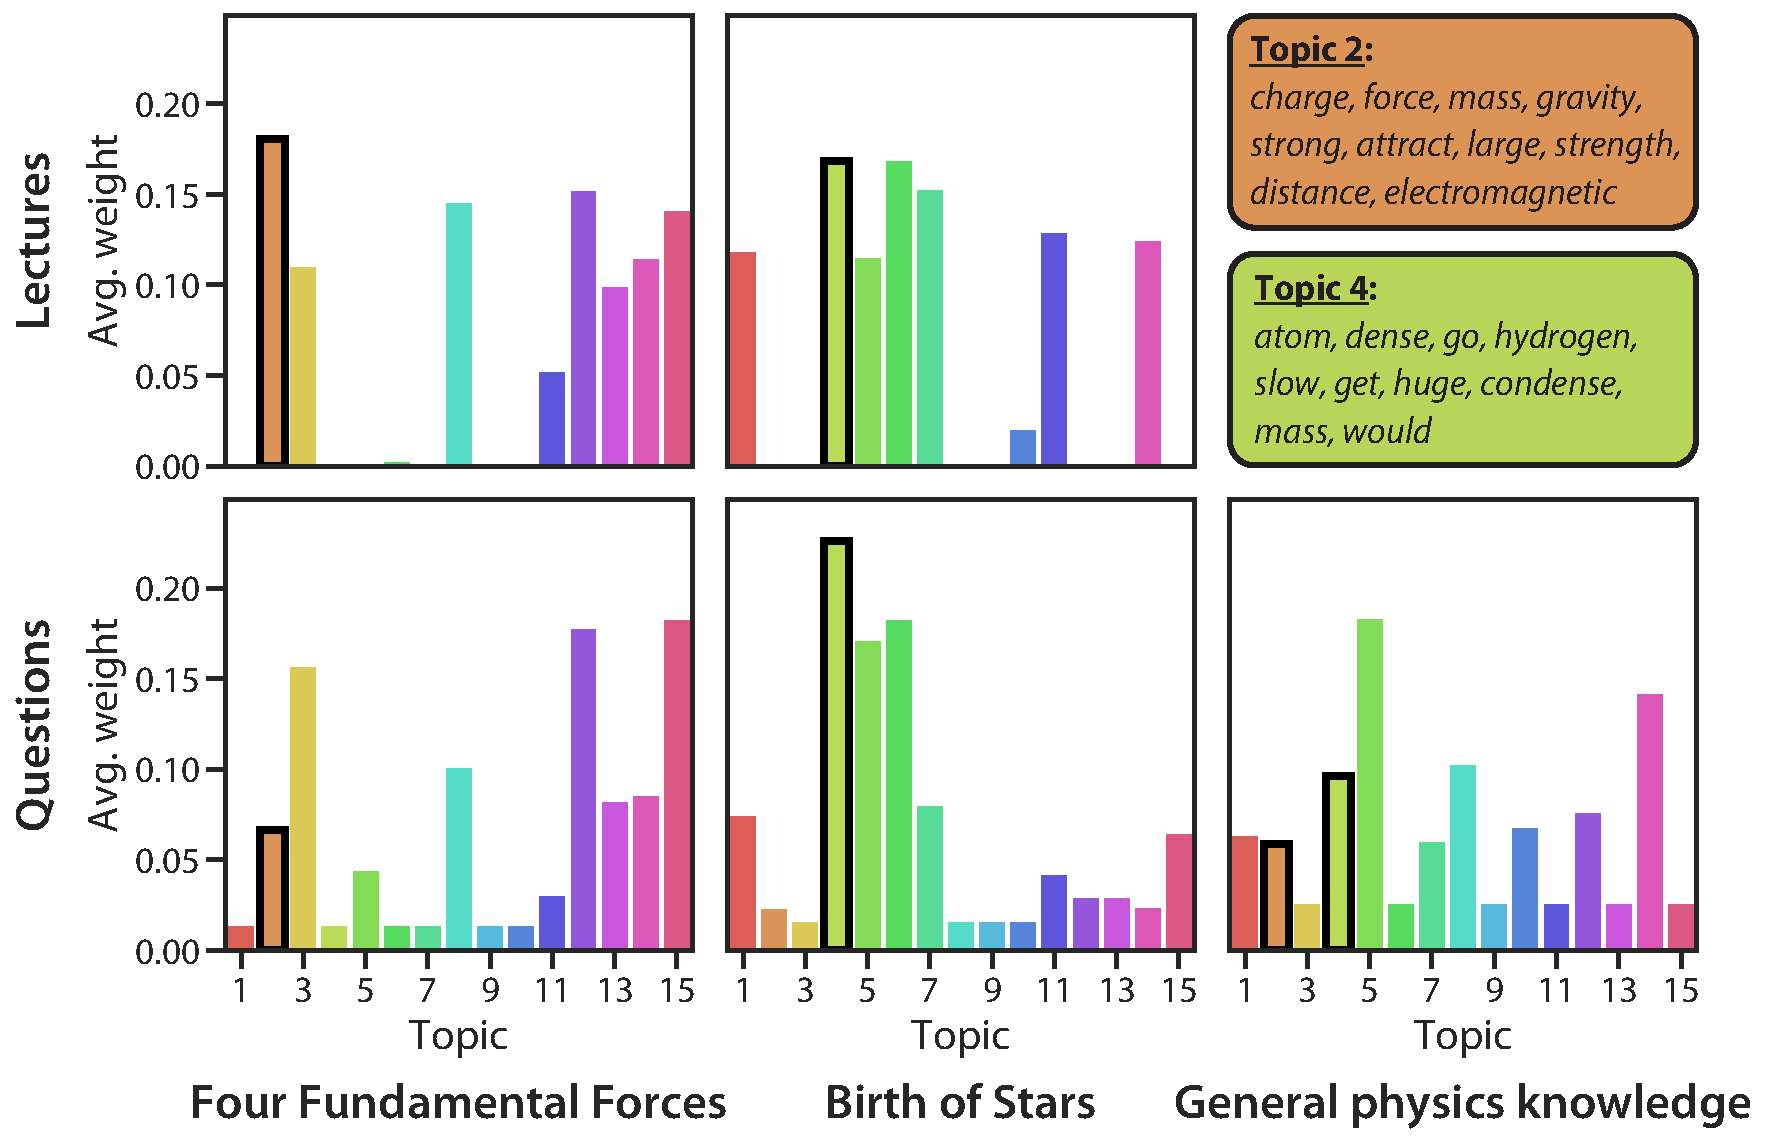
\includegraphics[width=\textwidth]{figs/topic-weights}

\caption{\textbf{Topic weights. A. Average topic weights for each lecture and
question type}. The bar plots display each topic's average weight across
lecture timepoints (top row) and questions (bottom row); colors denote topics.
The top-weighted words from the highest-weighted topic from each lecture are
displayed in the upper right (orange: topic 2; yellow-green: topic 4). The
top-weighted words from the full set of topics may be found in
Table~\ref{tab:topics}. \textbf{B. Relationships between average topic
weights.} Pairwise correlations between the distributions of average topic
weights for each lecture and question category. Each row and column corresponds
to a bar plot in Panel A. Also see Figure~\topics A in the main text.}

    \label{fig:topics}
\end{figure}

\newpage

\begin{figure}[tp]
    \centering
    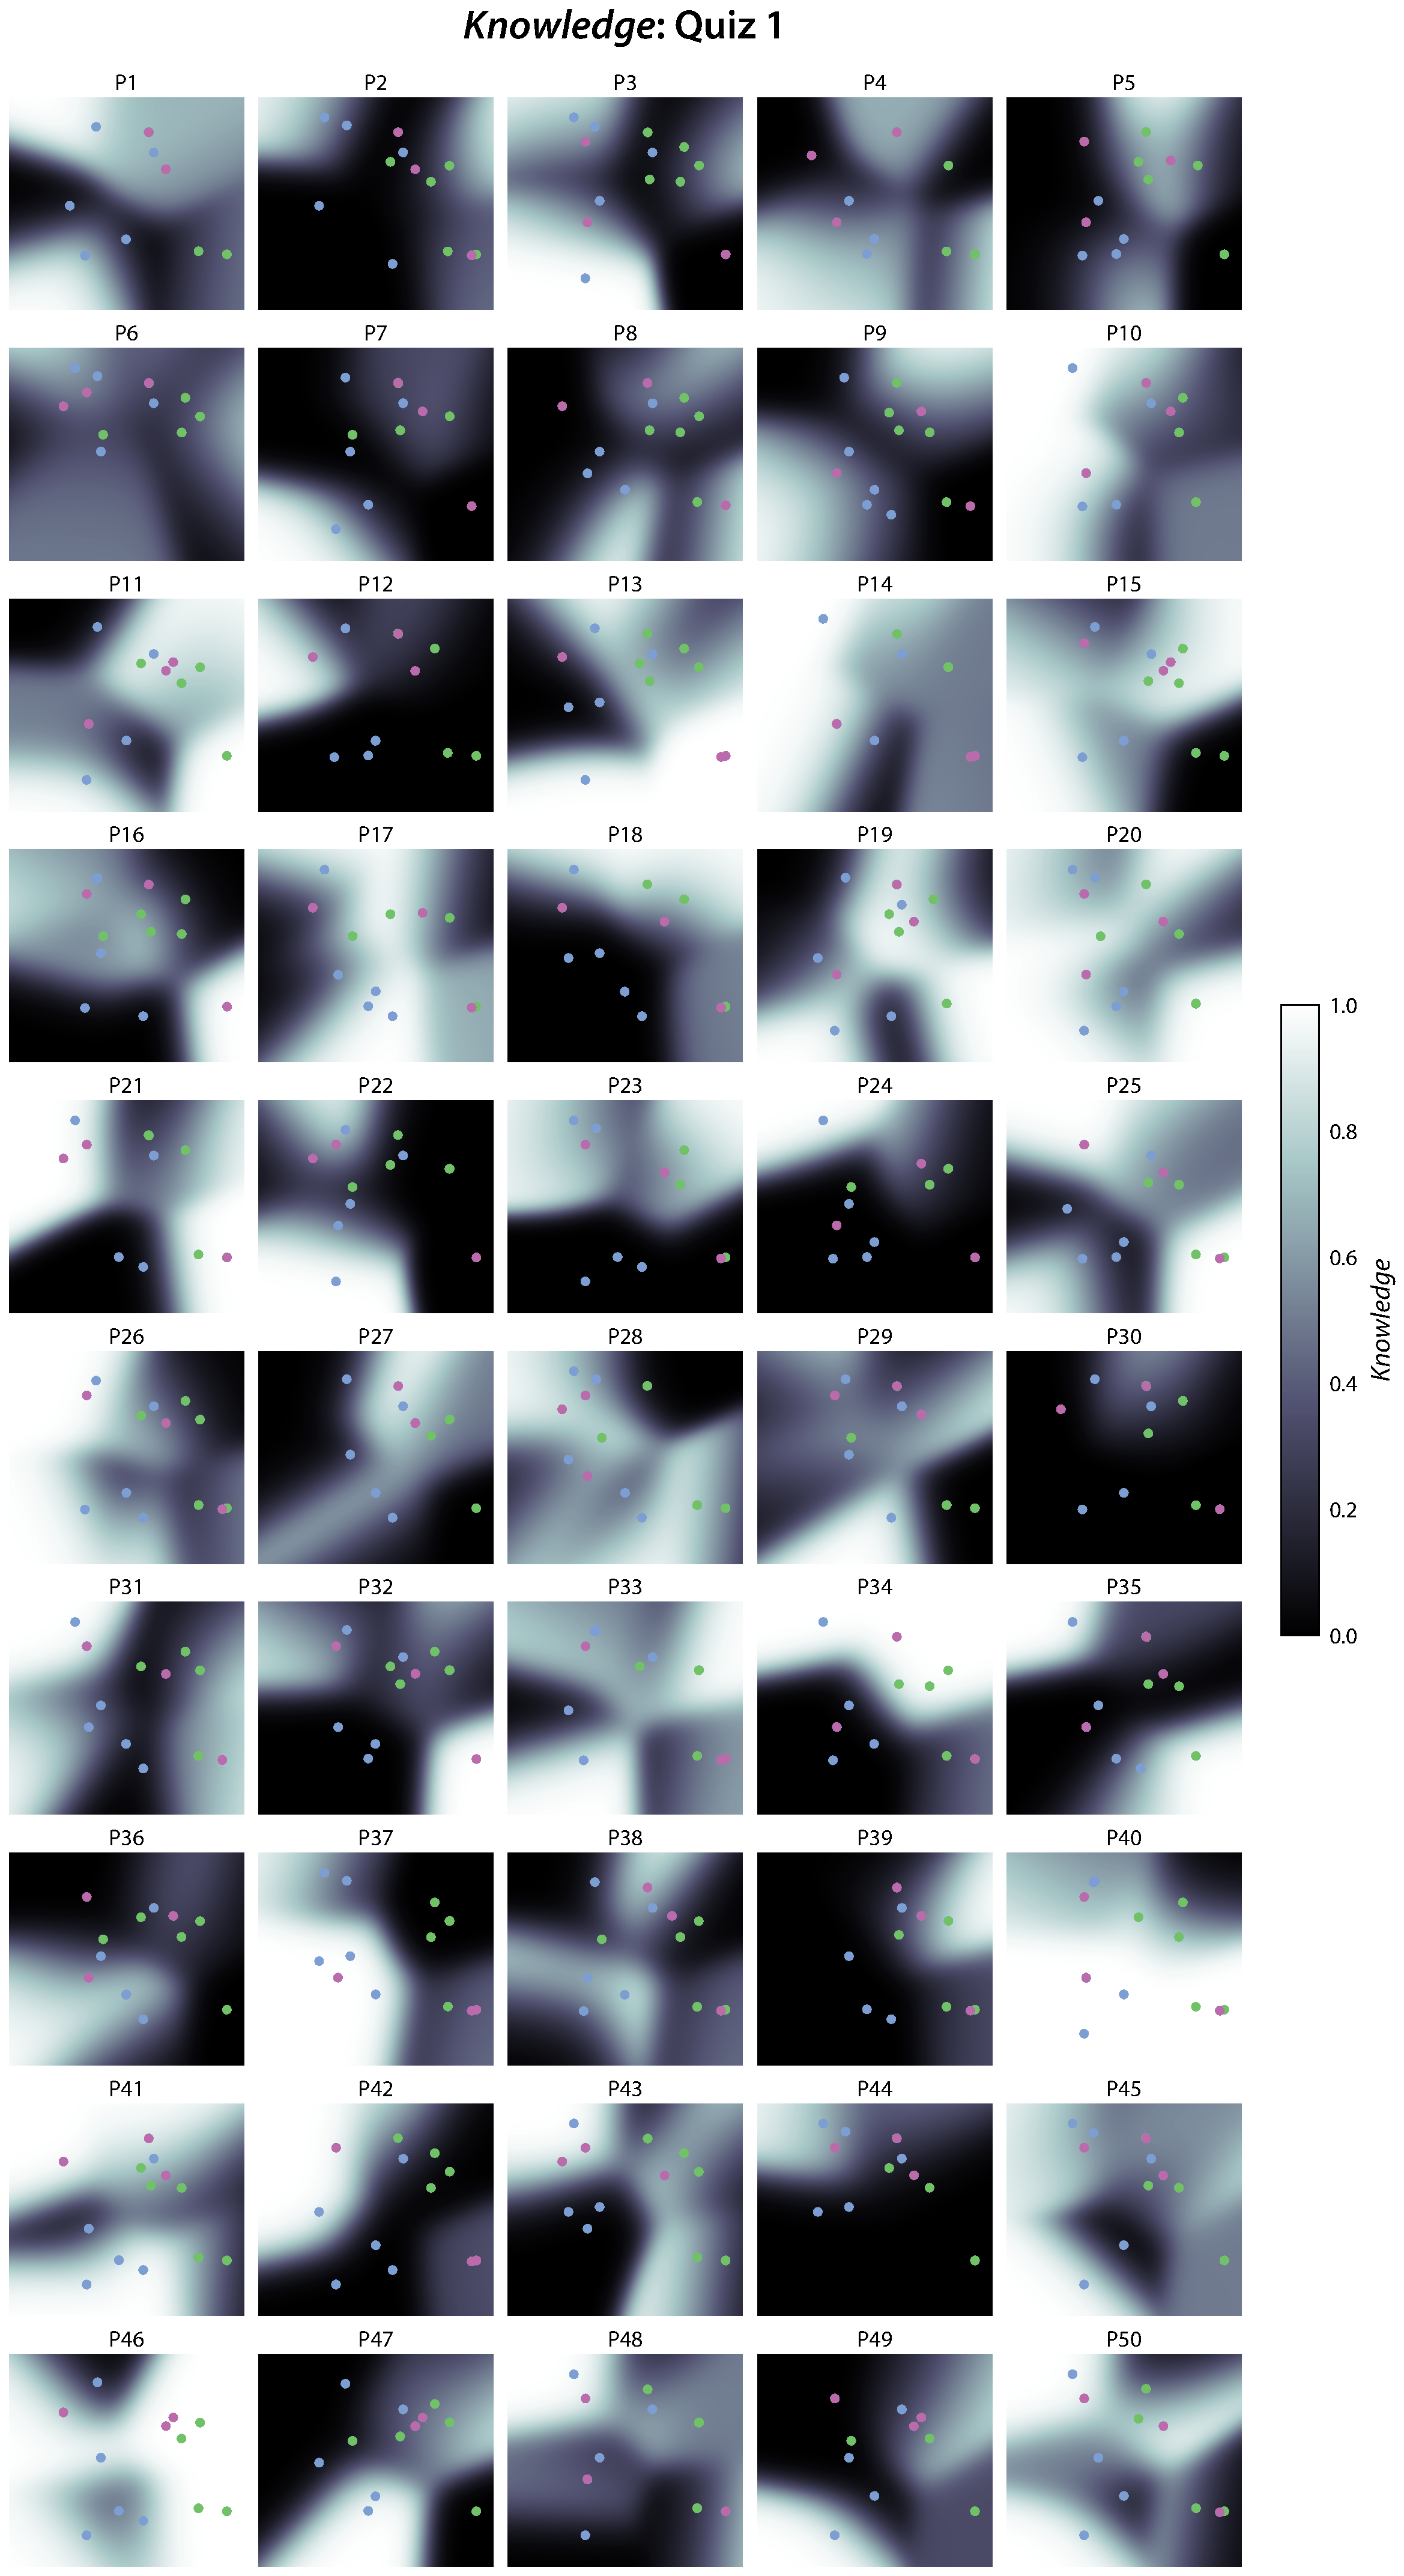
\includegraphics[height=0.9\textheight]{figs/individual-knowledge-maps-quiz1}
    
    \caption{\textbf{Individual participants' knowledge maps estimated from
    Quiz 1 responses.} Each panel is in the same format as the knowledge maps
    displayed in the left panel of Figure~\knowledgeMaps A in the main text,
    but here the maps have been computed separately for each participant.}
    
    \label{fig:knowledge-maps-q1}
\end{figure}

\begin{figure}[tp]
    \centering
    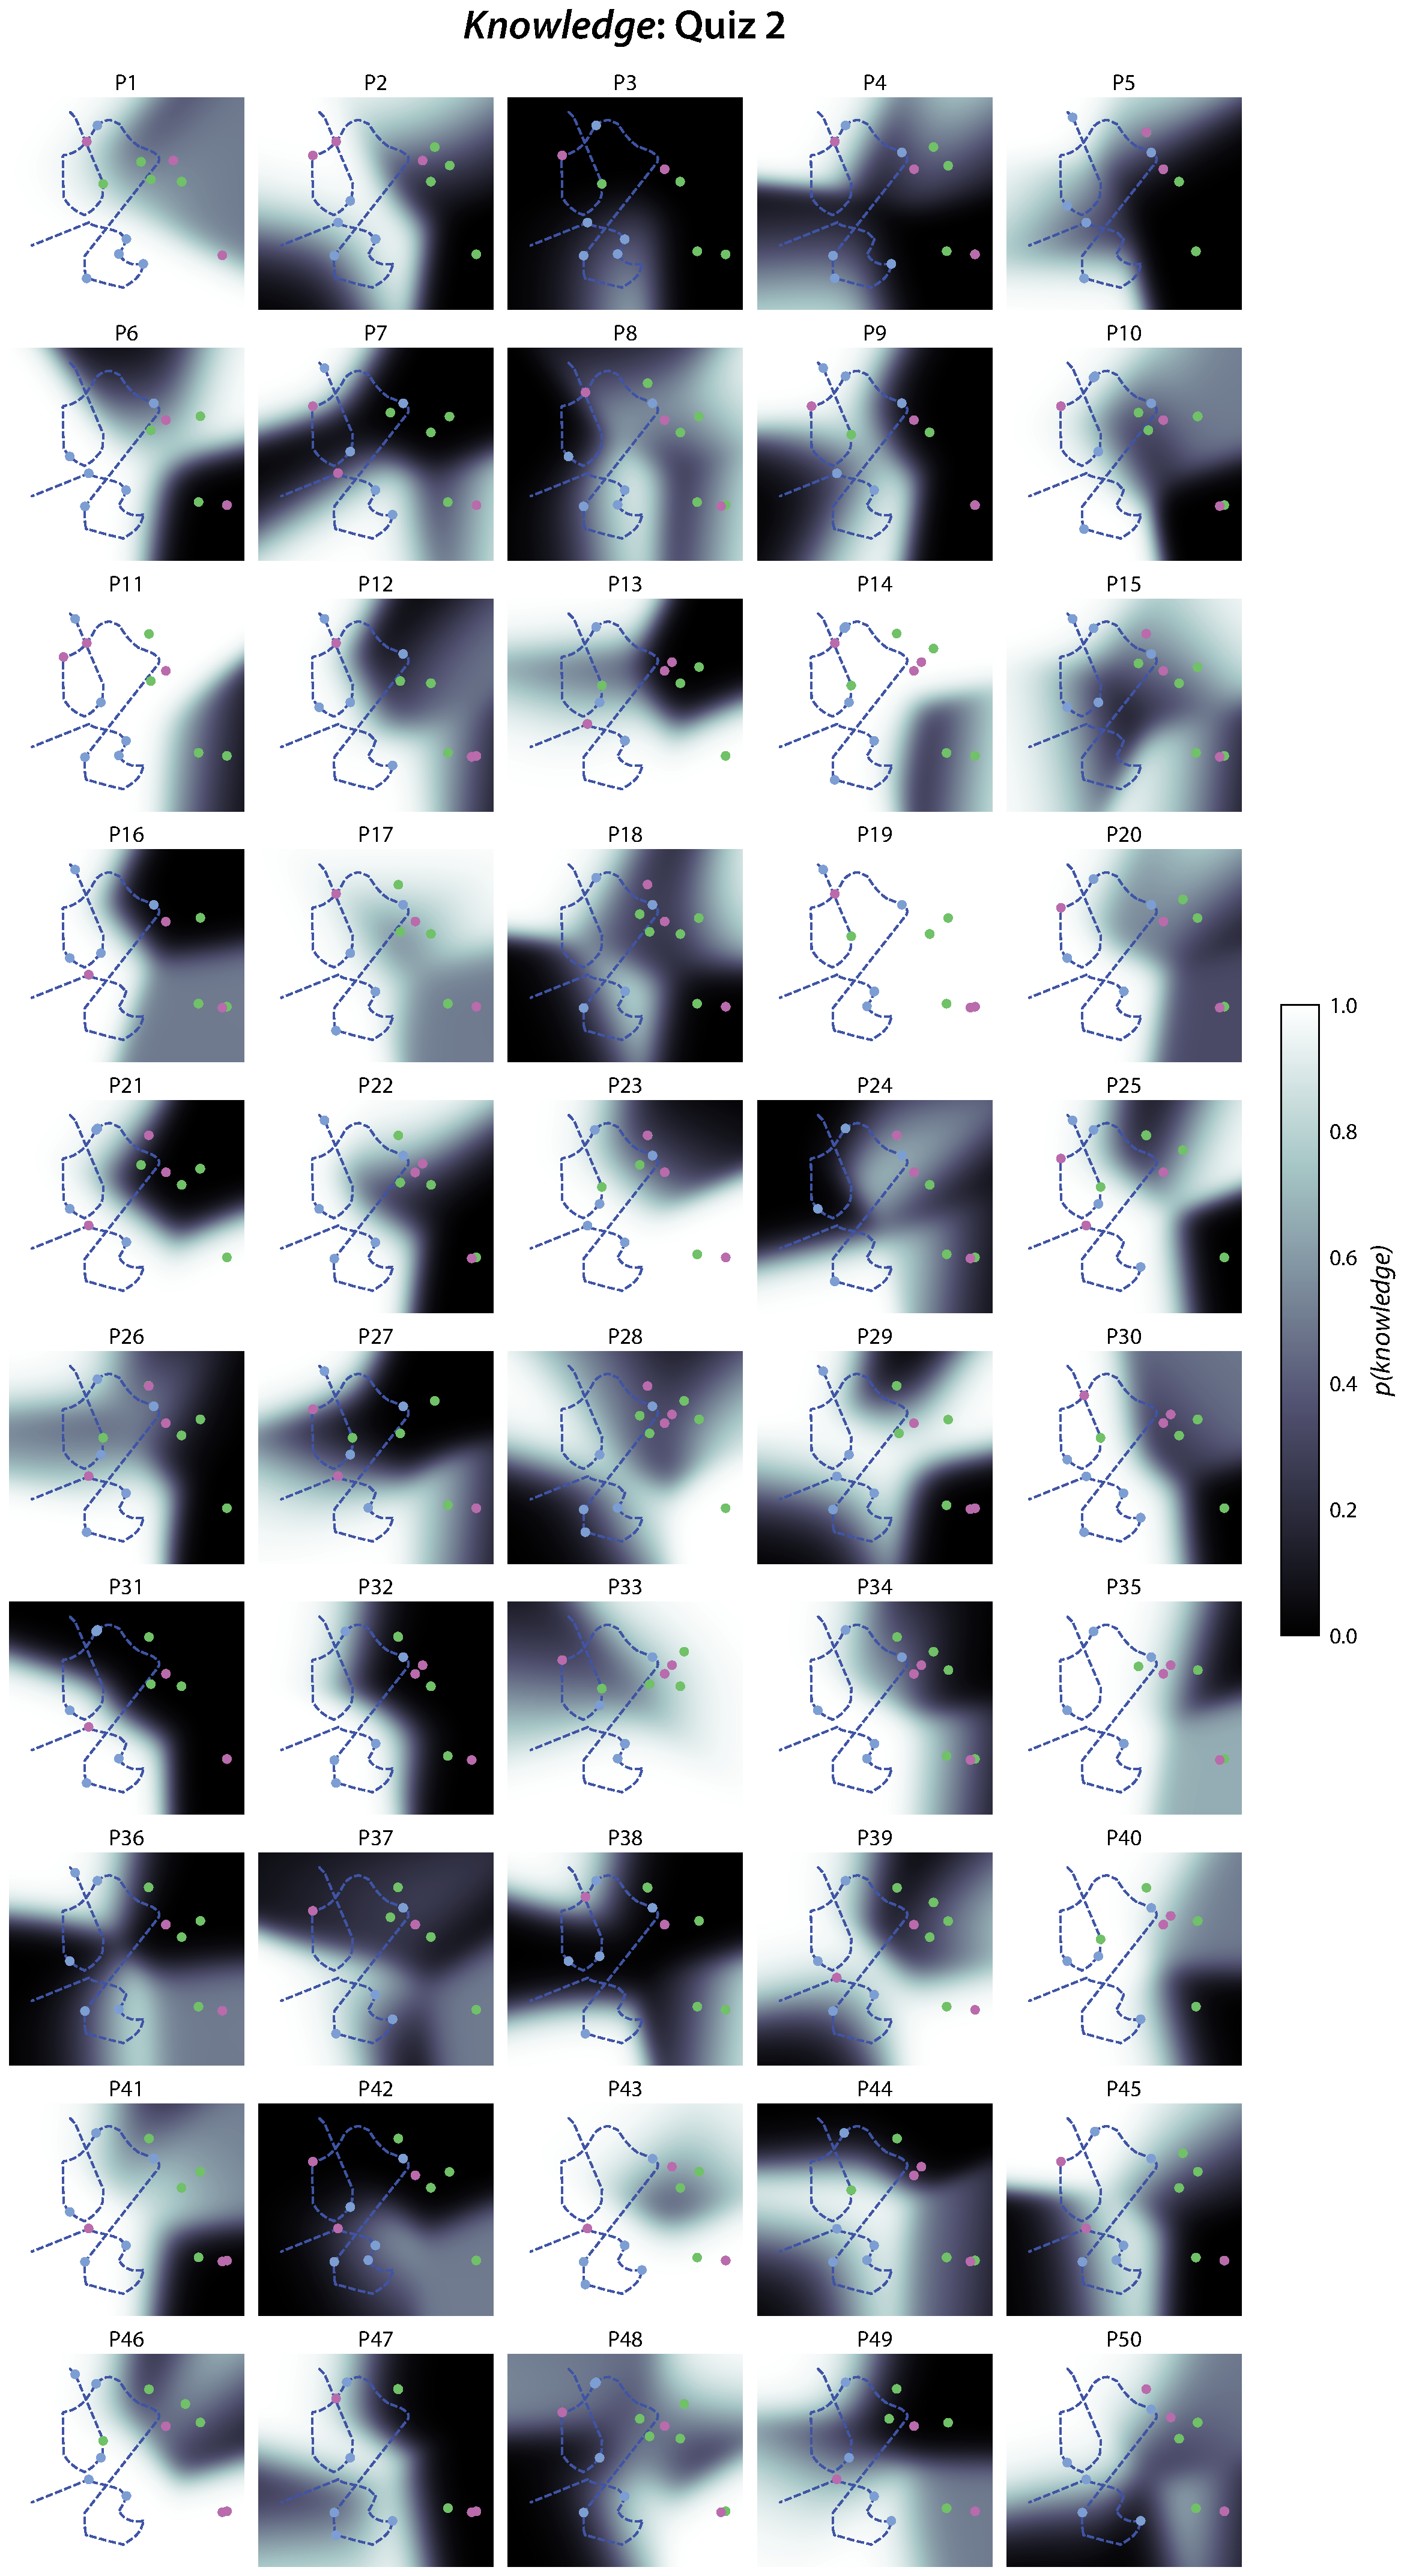
\includegraphics[height=0.9\textheight]{figs/individual-knowledge-maps-quiz2}
    
    \caption{\textbf{Individual participants' knowledge maps estimated from
    Quiz 2 responses.} Each panel is in the same format as the knowledge maps
    displayed in the middle panel of Figure~\knowledgeMaps A in the main text,
    but here the maps have been computed separately for each participant.}
    
    \label{fig:knowledge-maps-q2}
\end{figure}

\begin{figure}[tp]
    \centering
    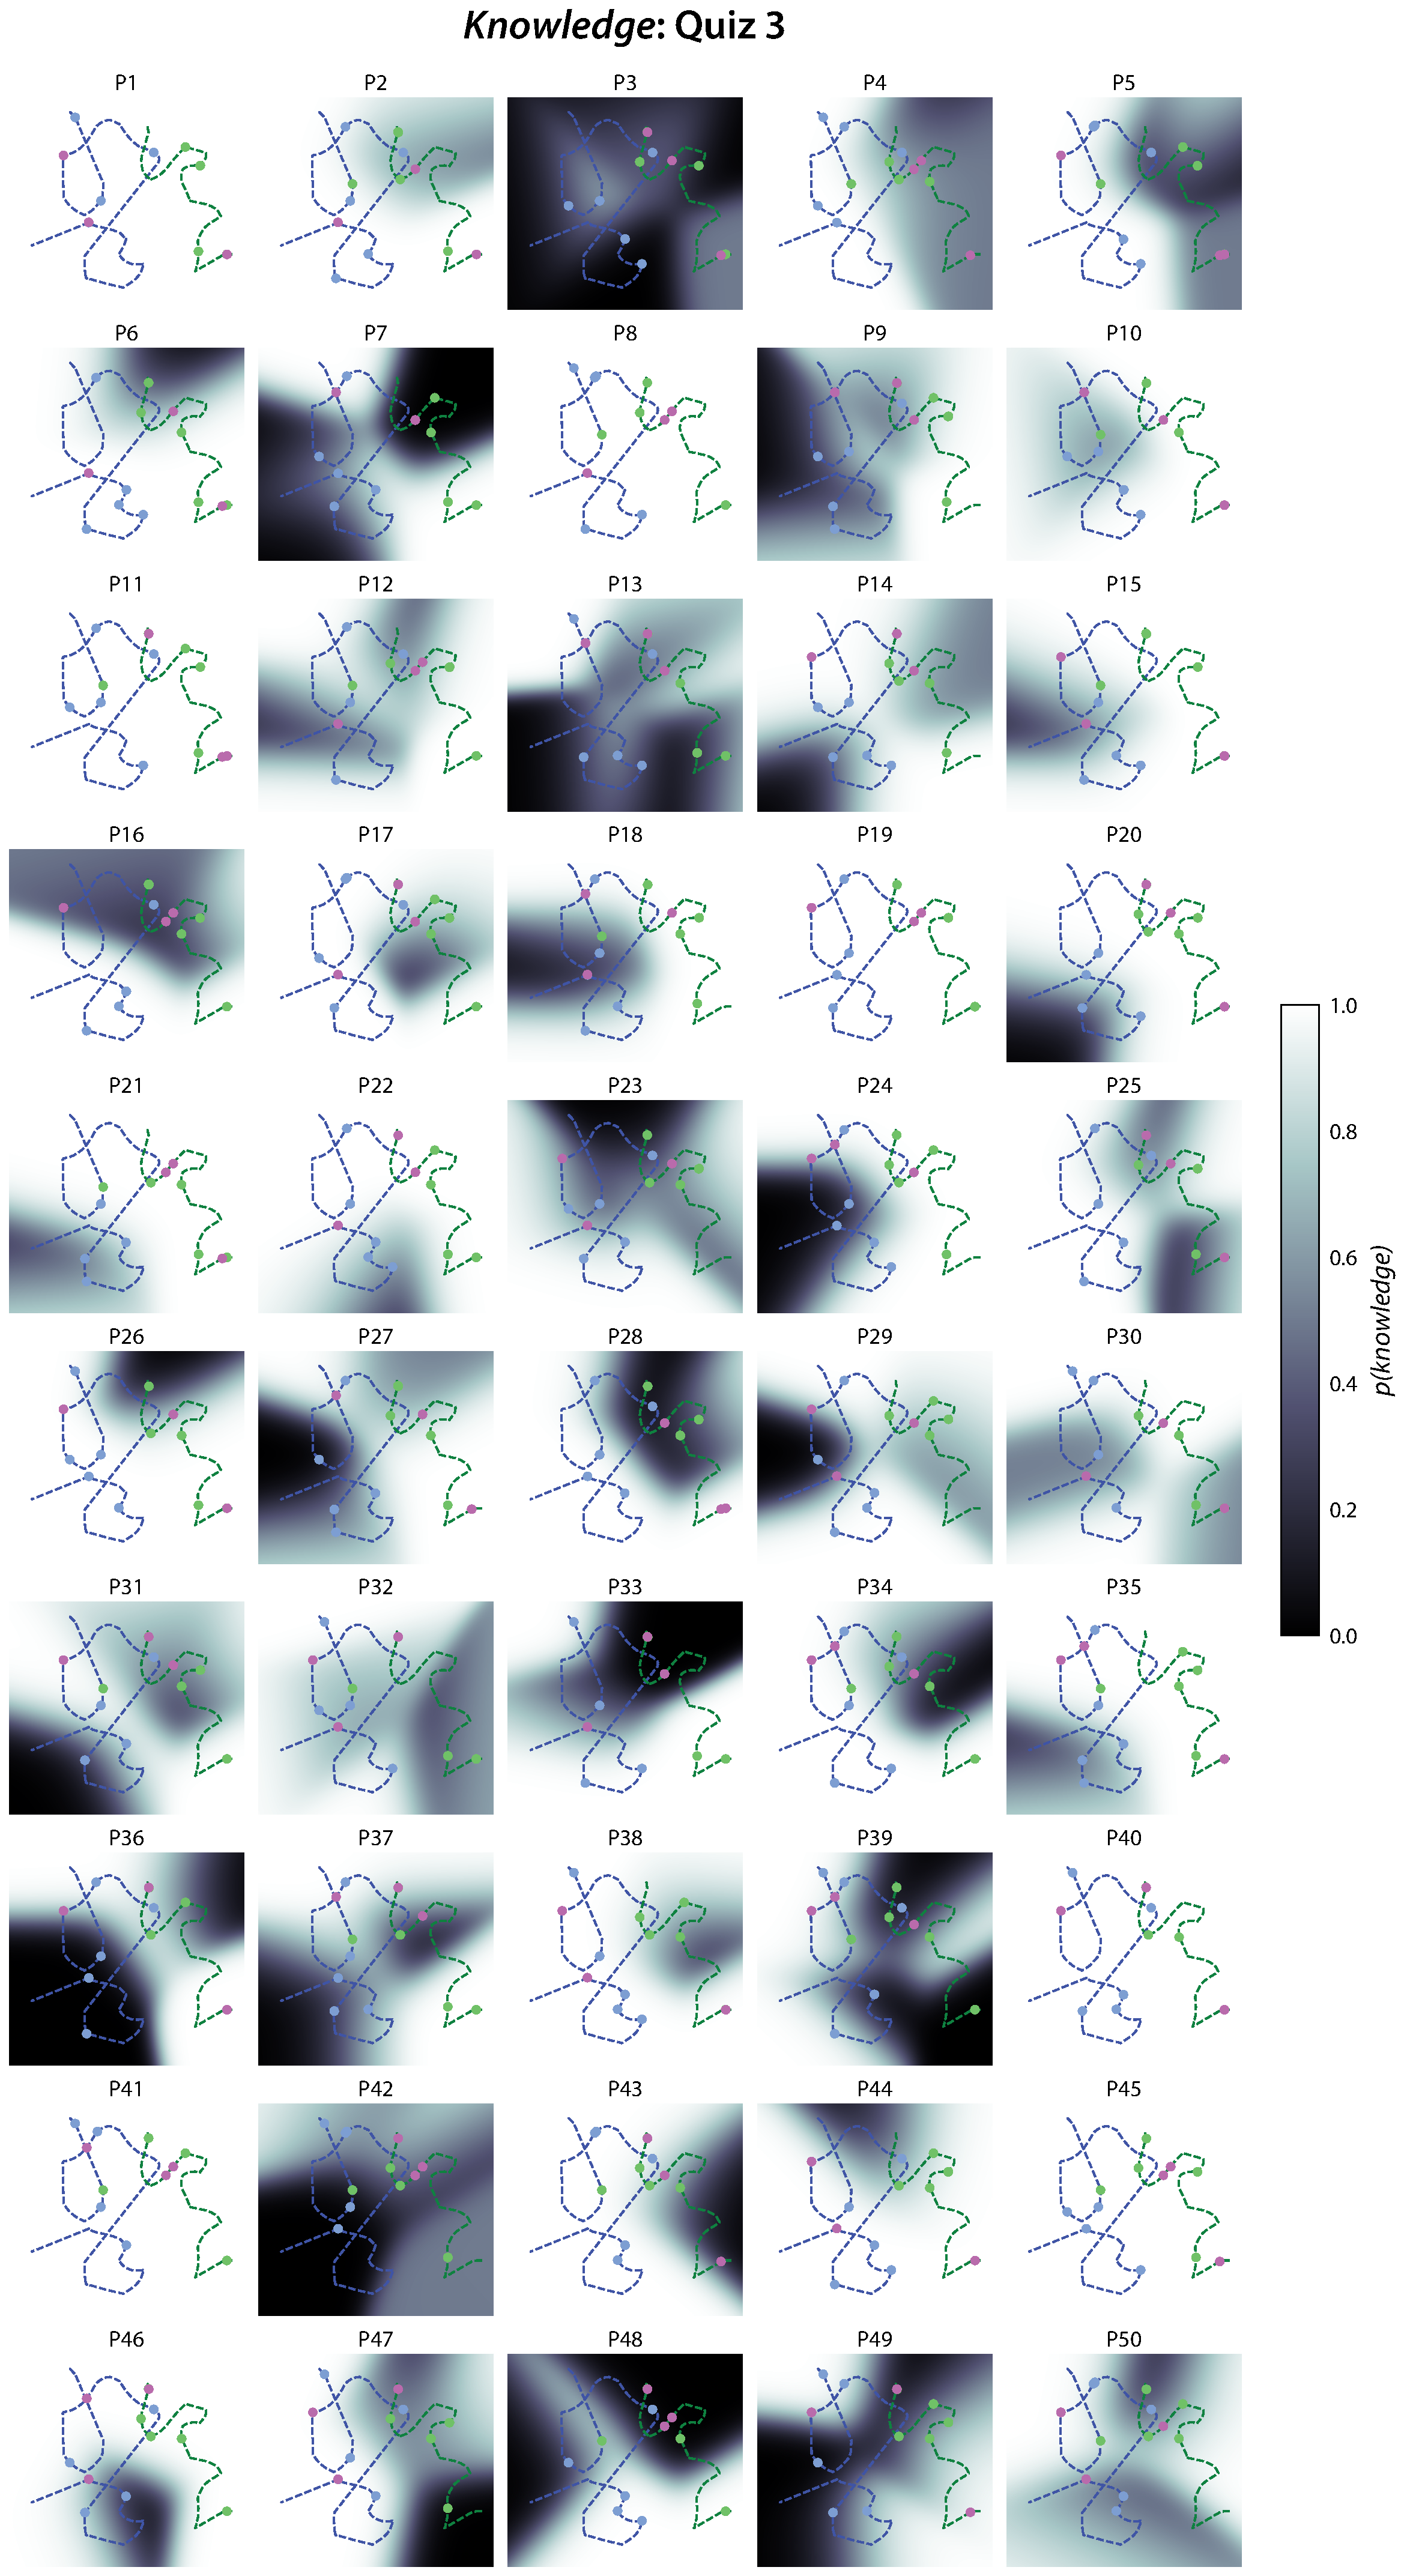
\includegraphics[height=0.9\textheight]{figs/individual-knowledge-maps-quiz3}
    
    \caption{\textbf{Individual participants' knowledge maps estimated from
    Quiz 3 responses.} Each panel is in the same format as the knowledge maps
    displayed in the right panel of Figure~\knowledgeMaps A in the main text,
    but here the maps have been computed separately for each participant.}
    
    \label{fig:knowledge-maps-q3}
\end{figure}

\begin{figure}[tp]
    \centering
    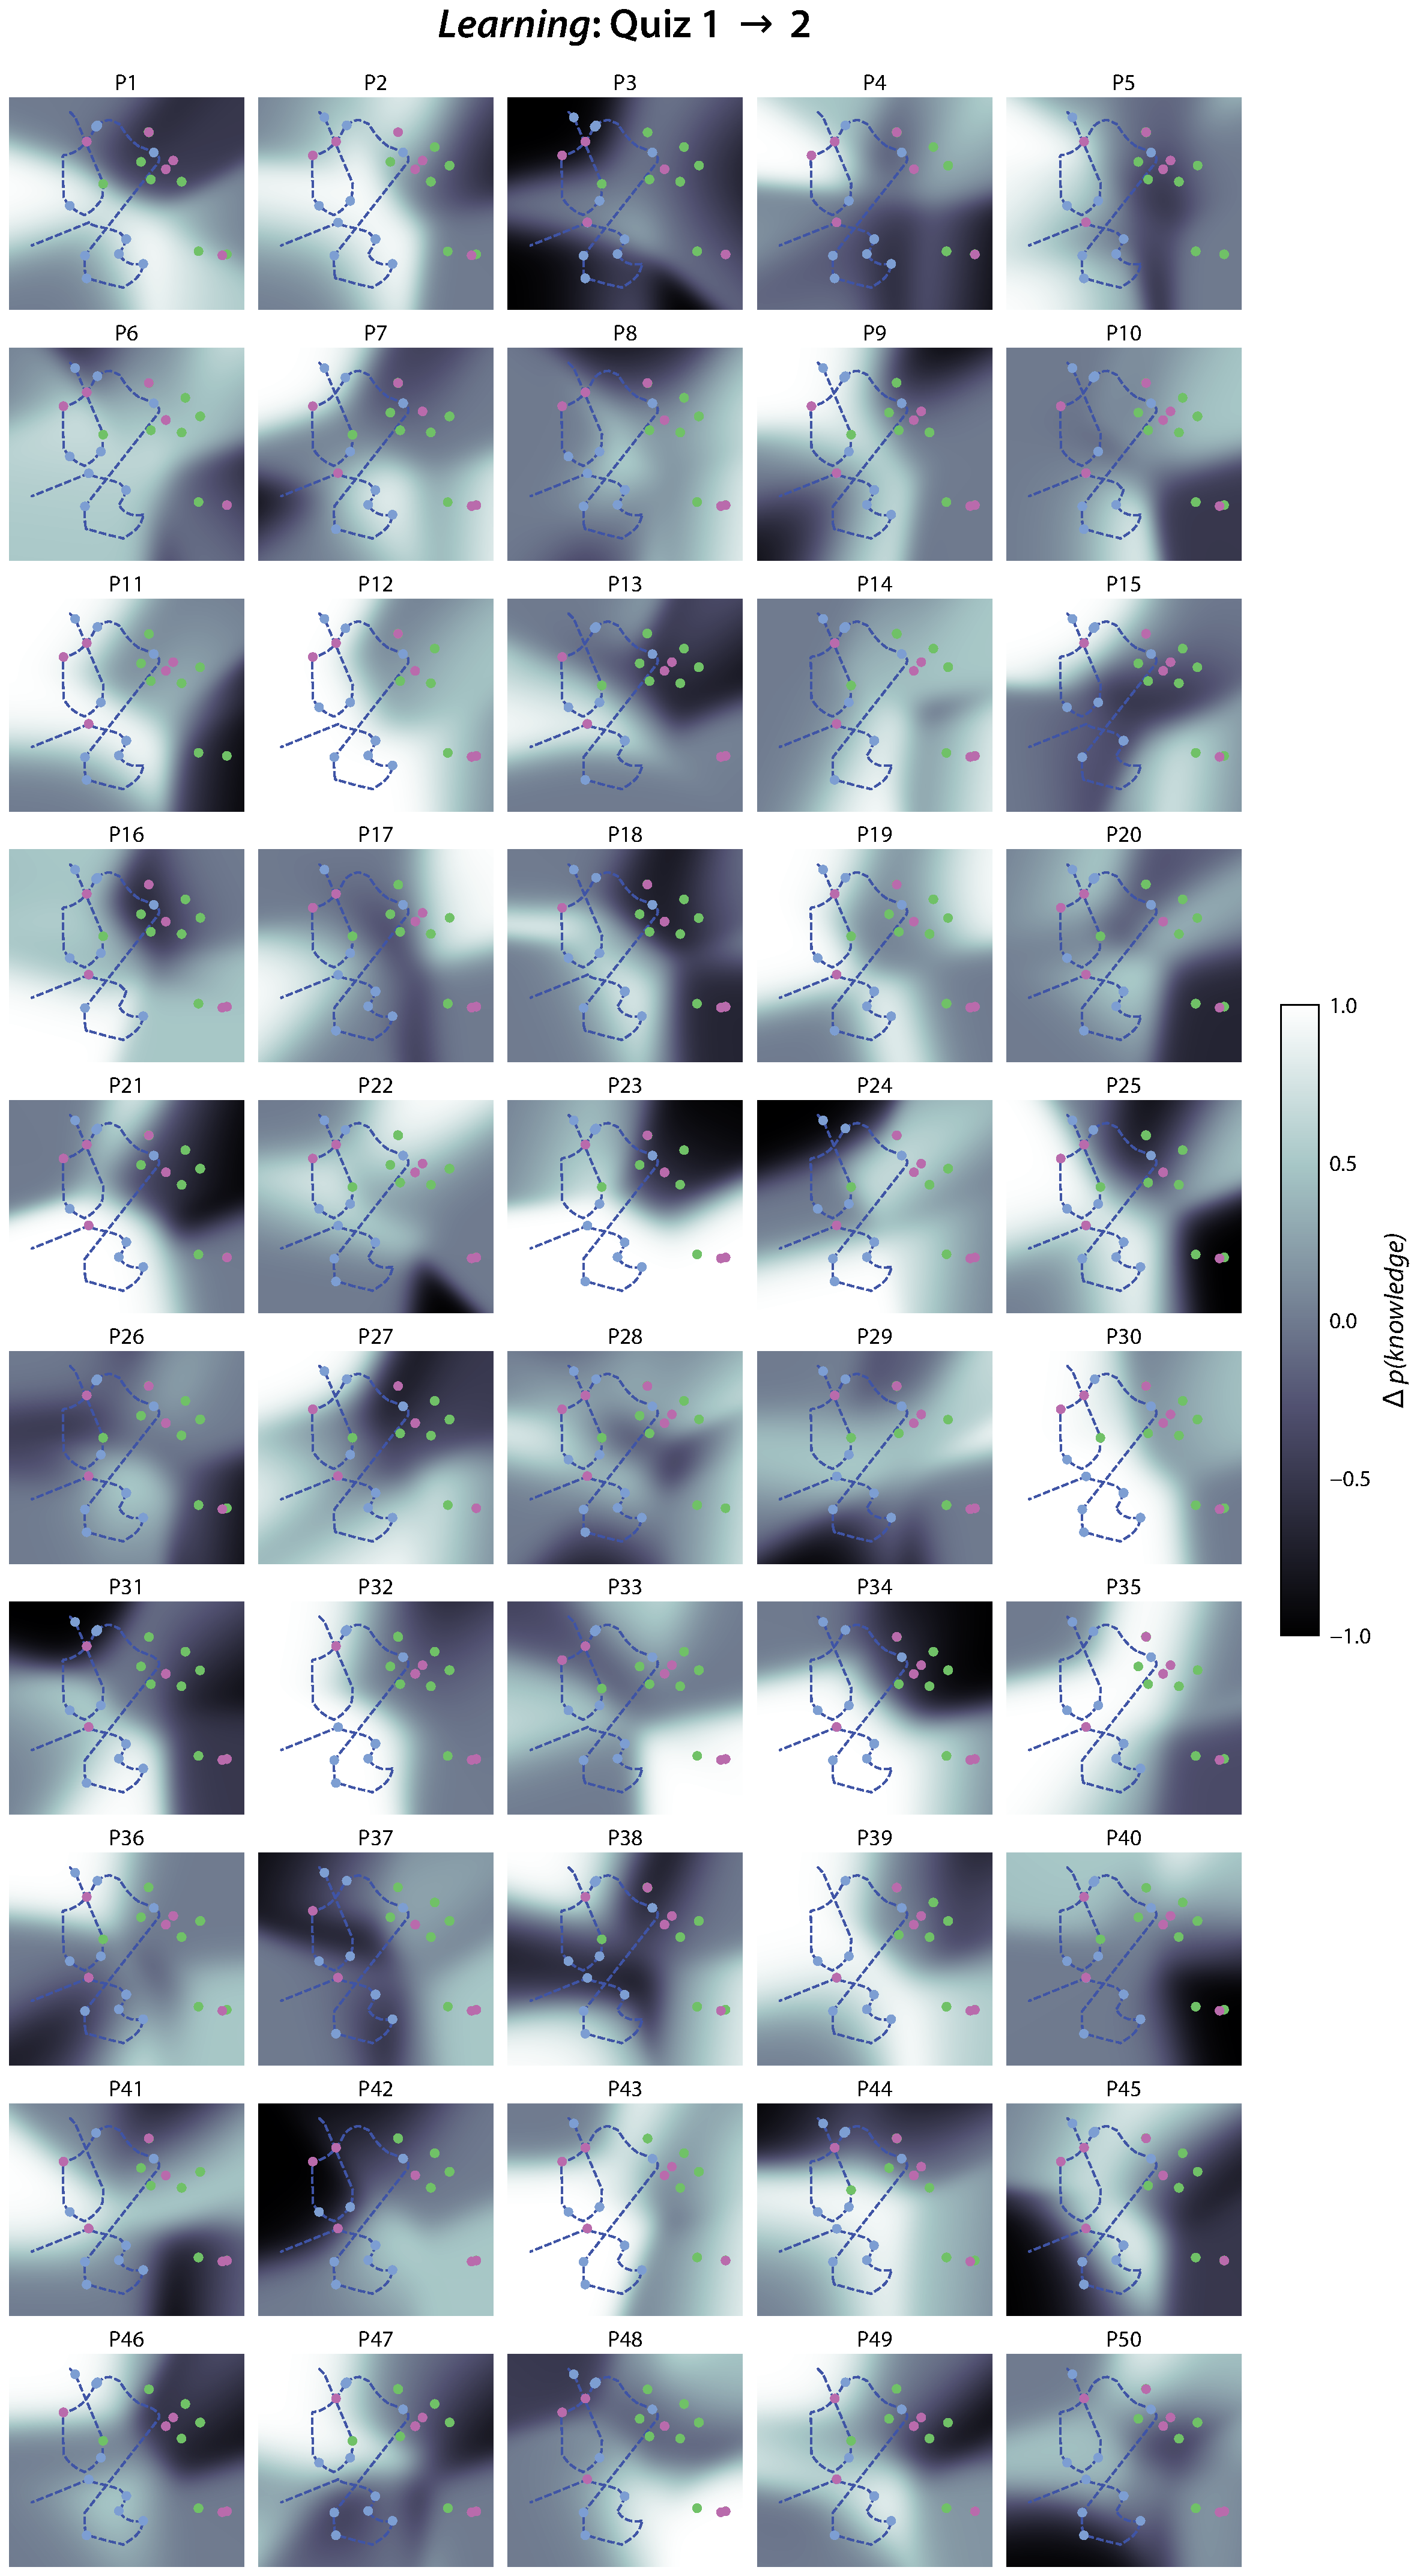
\includegraphics[height=0.9\textheight]{figs/individual-learnings-maps-quiz1-2}
    
    \caption{\textbf{Individual participants' learning maps estimated from
    Quiz 1 and 2 responses.} Each panel is in the same format as the learning map
    displayed in the left panel of Figure~\knowledgeMaps B in the main text,
    but here the maps have been computed separately for each participant.}
    
    \label{fig:learning-maps-q1_2}
\end{figure}

\begin{figure}[tp]
    \centering
    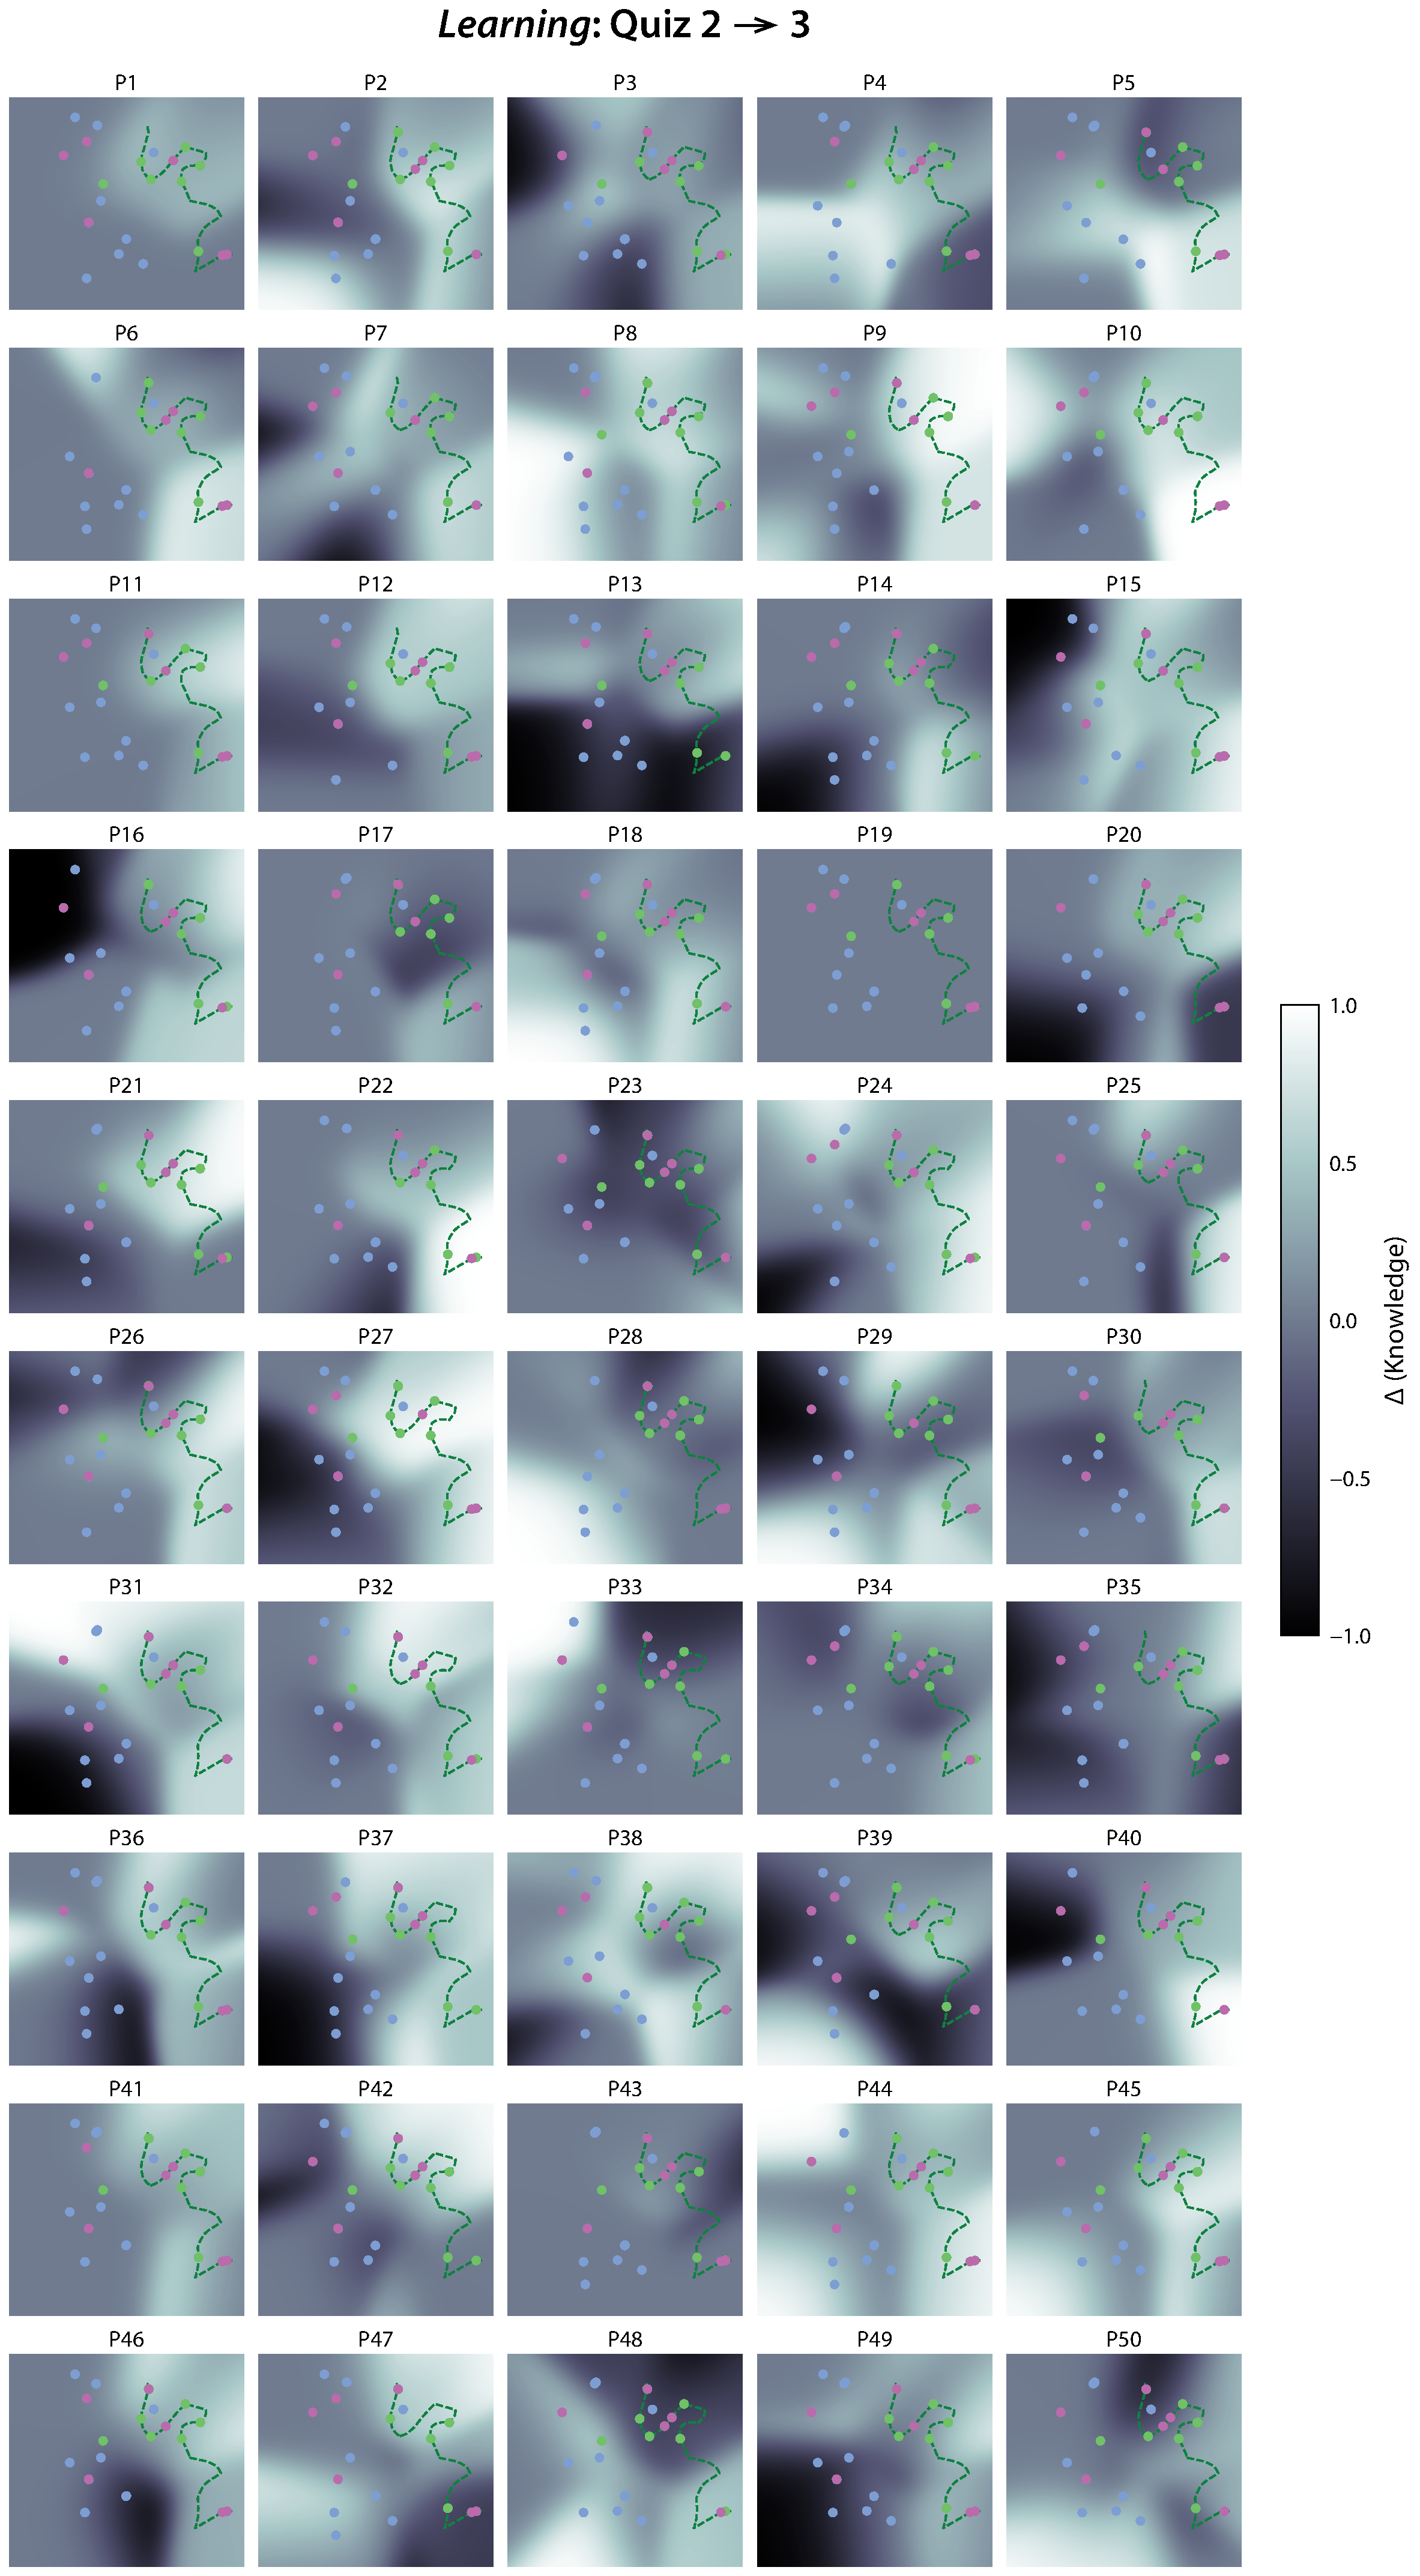
\includegraphics[height=0.9\textheight]{figs/individual-learnings-maps-quiz2-3}
    
    \caption{\textbf{Individual participants' learning maps estimated from
    Quiz 2 and 3 responses.} Each panel is in the same format as the learning map
    displayed in the right panel of Figure~\knowledgeMaps B in the main text,
    but here the maps have been computed separately for each participant.}
    
    \label{fig:learning-maps-q1_2}
\end{figure}


% \renewcommand{\refname}{Supplementary references}
% \bibliographystyle{apa}
% \bibliography{CDL-bibliography/cdl}



\end{document}
